% ----------------------------------------------------------
% ILLUSTRATIVE EXAMPLE
% ----------------------------------------------------------
\section{Illustrative Example}

Consider a single item evaluated over twelve consecutive intervals. For each
interval $t$, realized demand $y_t$ is compared with the corresponding forecast
$\yhat_t$, and a shortfall is recorded when $\yhat_t < y_t$.

Figure~\ref{fig:nsl_interval_coverage} illustrates the resulting interval-level
coverage pattern. Dark segments indicate intervals in which forecasted demand met
or exceeded realized demand, while unfilled segments indicate shortfall events.
The figure highlights the binary structure of the metric: each interval contributes
either a success or a failure, independent of error magnitude.

\begin{figure}[h!]
\centering
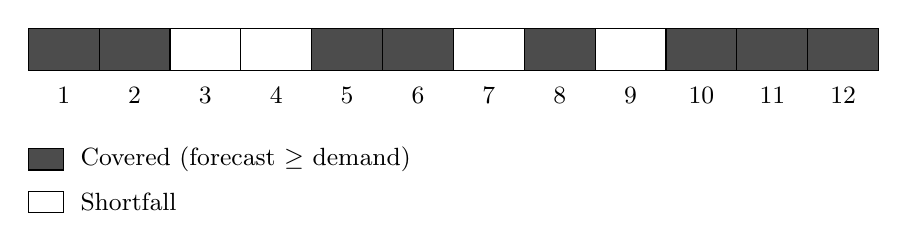
\begin{tikzpicture}[scale=0.9]

% ----------------------------------------------------------
% Covered intervals (forecast >= demand)
% ----------------------------------------------------------
\foreach \x in {0,1,4,5,7,9,10,11} {
    \draw[fill=black!70] (\x,0) rectangle ++(1,0.6);
}

% ----------------------------------------------------------
% Shortfall intervals
% ----------------------------------------------------------
\foreach \x in {2,3,6,8} {
    \draw[fill=white] (\x,0) rectangle ++(1,0.6);
    \draw (\x,0) rectangle ++(1,0.6);
}

% ----------------------------------------------------------
% Interval labels
% ----------------------------------------------------------
\foreach \x in {0,...,11} {
    \node at (\x+0.5,-0.35) {\small \the\numexpr\x+1\relax};
}

% ----------------------------------------------------------
% Legend
% ----------------------------------------------------------
\draw[fill=black!70] (0,-1.4) rectangle ++(0.5,0.3);
\node[right] at (0.6,-1.25) {\small Covered (forecast $\ge$ demand)};

\draw[fill=white] (0,-2.0) rectangle ++(0.5,0.3);
\draw (0,-2.0) rectangle ++(0.5,0.3);
\node[right] at (0.6,-1.85) {\small Shortfall};

\end{tikzpicture}
\caption{Interval-level coverage pattern illustrating \NSL\ for a 12-interval example.}
\label{fig:nsl_interval_coverage}
\end{figure}

Table~\ref{tab:nsl_example} reports the underlying realized demand values, forecasts,
and shortfall indicators for each interval. Shortfalls occur in intervals 2, 3, 5,
7, and 9, while demand is adequately covered in the remaining intervals.

\input{tables/050_nsl_intervals_example}

The resulting No-Shortfall Level is therefore
\[
\NSL = \frac{7}{12} \approx 0.583.
\]

This value indicates that demand was met in approximately 58 percent of intervals.
The example also illustrates a defining characteristic of the metric: \NSL\ is
unaffected by the size of shortfalls or surpluses, focusing exclusively on their
occurrence. Two forecasts with identical \NSL\ values may therefore differ
substantially in error magnitude, motivating the complementary use of magnitude-
based metrics alongside \NSL.